% =====================================================================
% dfl_explainer.tex
%
% Visual walkthrough of the Decision-Focused Learning (DFL) approach for
% the Discrete Berth Allocation Problem (DBAP) at Puerto de San Antonio.
% Audience: engineering PhD / committee; assumes optimization background
% but NOT prior DFL exposure.  Each tikzpicture is a single page so any
% block can be lifted into a Beamer slide.
%
% Build:  pdflatex dfl_explainer.tex  (twice, for cross references)
%
% Source of truth for labels and formulas:
%   prediction_models/src/ports_dfl/train/pto.py
%   prediction_models/src/ports_dfl/train/dfl_blackbox.py
%   prediction_models/src/ports_dfl/train/dfl_perturbed.py
%   prediction_models/src/ports_dfl/optim/discrete_bap.py
%   prediction_models/src/ports_dfl/optim/classic_bap.py
% =====================================================================
\documentclass[11pt]{article}

\usepackage[landscape, margin=0.6in]{geometry}
\usepackage{tikz}
\usepackage{pgfplots}
\pgfplotsset{compat=1.18}
\usepackage{amsmath, amssymb}
\usepackage{booktabs}
\usepackage{caption}
\usepackage{xcolor}
\usepackage{enumitem}

\usetikzlibrary{
  positioning,
  arrows.meta,
  fit,
  calc,
  backgrounds,
  shapes.geometric,
  decorations.pathreplacing
}

% ---------------------------------------------------------------------
% Color palette
% ---------------------------------------------------------------------
\definecolor{dataGray}{HTML}{5C6770}
\definecolor{predBlue}{HTML}{2C6FA8}
\definecolor{optOrange}{HTML}{D97706}
\definecolor{truthGreen}{HTML}{2E8B57}
\definecolor{regretRed}{HTML}{B23A48}

% ---------------------------------------------------------------------
% Reusable TikZ styles
% ---------------------------------------------------------------------
\tikzset{
  data/.style    = {rectangle, rounded corners=2pt, draw=dataGray,
                    fill=dataGray!8, line width=0.7pt,
                    minimum width=2.4cm, minimum height=0.8cm,
                    align=center, font=\small},
  pred/.style    = {rectangle, draw=predBlue, fill=predBlue!10,
                    line width=1pt, minimum width=2.4cm, minimum height=0.8cm,
                    align=center, font=\small},
  opt/.style     = {rectangle, draw=optOrange, fill=optOrange!12,
                    line width=1pt, minimum width=2.4cm, minimum height=0.8cm,
                    align=center, font=\small},
  optbb/.style   = {rectangle, draw=optOrange, fill=optOrange!12,
                    line width=1pt, double, double distance=1.5pt,
                    minimum width=2.4cm, minimum height=0.8cm,
                    align=center, font=\small},
  decision/.style= {rectangle, rounded corners=2pt, draw=truthGreen,
                    fill=white, line width=1pt,
                    minimum width=2.4cm, minimum height=0.8cm,
                    align=center, font=\small},
  truth/.style   = {rectangle, rounded corners=2pt, draw=truthGreen,
                    dashed, fill=truthGreen!8, line width=0.9pt,
                    minimum width=2.4cm, minimum height=0.8cm,
                    align=center, font=\small},
  regret/.style  = {rectangle, draw=regretRed, fill=regretRed!10,
                    line width=1pt, minimum width=2.4cm, minimum height=0.8cm,
                    align=center, font=\small},
  arrow/.style   = {-{Stealth[length=2mm]}, thick, draw=black!70},
  truthArrow/.style = {-{Stealth[length=2mm]}, thick, dashed, draw=truthGreen},
  gradArrow/.style  = {-{Stealth[length=2mm]}, thick, dashed, draw=regretRed},
  note/.style    = {font=\footnotesize\itshape, text=dataGray},
  panel/.style   = {rounded corners=4pt, draw=dataGray!40,
                    line width=0.5pt, inner sep=8pt}
}

\captionsetup{labelformat=empty, font=small}

% ---------------------------------------------------------------------
\begin{document}

% =====================================================================
% Title page
% =====================================================================
\begin{center}
{\Large\bfseries Decision-Focused Learning for Berth Allocation}\\[4pt]
{\small Puerto de San Antonio, Chile \;\textbar\;
        meeting walkthrough}
\end{center}

\vspace{0.6em}

\noindent
These figures explain paper 3 of the dissertation.  Assumes
optimization background; no prior DFL exposure required.  All formulas
trace to the code in \texttt{prediction\_models/}.

\vspace{1em}

\noindent\textbf{Contents.}
\begin{enumerate}[leftmargin=2em, itemsep=0pt]
  \item Figure 2.\ The MILP we solve.
  \item Figure 2c.\ The classical discrete BAP from the literature.
  \item Figure 2d.\ Alternatives to DFL.
  \item Figure 4.\ PtO, DFL, and how we score them \emph{(the main figure)}.
  \item Figure 5b.\ How the test problems are built.
  \item Figure 5c.\ The blackbox gradient (Pogan\v{c}i\'c et al., 2020).
  \item Figure 5d.\ The Gaussian-perturbed gradient (Berthet et al., 2020).
  \item Figure 6.\ Where DFL pays off.
\end{enumerate}

\newpage

% =====================================================================
% Figure 2 -- The MILP we actually solve
% =====================================================================
\section*{Figure 2.\quad The MILP we solve}

\noindent
The berth-allocation MILP that runs inside every training step and at
evaluation time. Source:
\texttt{prediction\_models/src/ports\_dfl/optim/discrete\_bap.py}.

\vspace{0.5em}

\noindent\textbf{Sets.}
$\mathcal{I}=\{1,\dots,N\}$ vessels;\;
$\mathcal{B}=\{1,\dots,B\}$ berths.

\smallskip
\noindent\textbf{Parameters.}
$a_i$ arrival time of vessel $i$;\;
$w_i\geq 0$ priority weight;\;
$\tau_i\geq 0$ service time (the predictor's output, plugged in as a
mutable parameter);\;
$M$ big-M (horizon plus a slack so any single-berth schedule fits).

\smallskip
\noindent\textbf{Decision variables.}
$x_{ib}\in\{0,1\}$ is $1$ iff vessel $i$ is processed at berth $b$;\;
$s_i\in\mathbb{R}_{\geq 0}$ start time of vessel $i$;\;
$z_{ijb}\in\{0,1\}$ is $1$ iff $i$ precedes $j$ at berth $b$ (defined
for ordered pairs $i\neq j$).

\vspace{0.4em}

\begin{center}
\renewcommand{\arraystretch}{1.35}
\begin{tabular}{@{}r l l@{}}
\toprule
& \multicolumn{1}{c}{Expression} & \multicolumn{1}{c}{Meaning} \\
\midrule
$\displaystyle\min_{x,s,z}$ &
$\displaystyle\sum_{i\in\mathcal{I}} w_i\,(s_i + \tau_i)$ &
total weighted completion time \\
\midrule
s.t.\ &
$\displaystyle\sum_{b\in\mathcal{B}} x_{ib} = 1$ &
each vessel assigned to exactly one berth \\
&
$s_i \geq a_i$ &
no vessel starts before it arrives \\
&
$z_{ijb} + z_{jib} \leq 1$ &
at most one direction of precedence per pair-berth \\
&
$z_{ijb} + z_{jib} \geq x_{ib} + x_{jb} - 1$ &
two vessels sharing a berth must be sequenced \\
&
$s_j \geq s_i + \tau_i - M\,(1 - z_{ijb})$ &
big-M precedence: if $z_{ijb}{=}1$, $j$ starts after $i$ finishes \\
&
$x_{ib},\, z_{ijb} \in \{0,1\},\; s_i \geq 0$ & \\
\bottomrule
\end{tabular}
\end{center}

\vspace{0.6em}

\noindent\textbf{Where $\tau$ enters.}
$\tau$ appears in both the objective and the precedence constraints.
At training time the solver receives $\hat{\tau}=f_\theta(x)$ in place
of $\tau$; at evaluation time start times are recomputed under the
true $\tau$ on the locked $(x,z)$ decision, so regret is always
non-negative.

\vspace{0.3em}

\noindent\textbf{Notes.}
In scheduling terms this is $\mathrm{P}\,|\,r_j\,|\,\sum w_j C_j$ in
Graham notation: berths as identical parallel machines, arrivals as
release dates, no due dates. Solved with Gurobi via Pyomo; $\tau$ is
a mutable Pyomo \texttt{Param} so each DFL training step updates
values rather than rebuilding the model.

\newpage

% =====================================================================
% Figure 2c -- Classical discrete BAP (Cordeau, Laporte, Legato, Moccia 2005)
% =====================================================================
\section*{Figure 2c.\quad The classical discrete BAP from the literature}

\noindent
What the operations-research literature actually calls the discrete
dynamic Berth Allocation Problem (DBAP). Reference formulation:
Cordeau, Laporte, Legato \& Moccia, ``Models and tabu search heuristics
for the berth-allocation problem,'' \emph{Transportation Science}
39(4):526--538, 2005 (``DBAP1''). Compared with Figure~2, the
classical model differs in four places, each highlighted below.

\vspace{0.5em}

\noindent\textbf{Sets.}
$\mathcal{I}=\{1,\dots,N\}$ vessels;\;
$\mathcal{B}=\{1,\dots,B\}$ berths.

\smallskip
\noindent\textbf{Parameters.}
$a_i$ arrival time;\;
$b_i$ departure deadline (time window) \textsc{[new]};\;
$w_i\geq 0$ priority weight;\;
$\tau_{ib}\geq 0$ service time of vessel $i$ \emph{at berth $b$}
\textsc{[berth-dependent, new]};\;
$M$ big-M constant.

\smallskip
\noindent\textbf{Decision variables.}
$y_{ib}\in\{0,1\}$ vessel--berth assignment;\;
$T_i\in\mathbb{R}_{\geq 0}$ berthing (start) time;\;
$D_i\in\mathbb{R}_{\geq 0}$ departure time;\;
$\sigma_{ij}\in\{0,1\}$ \emph{cross-berth} precedence: $1$ iff $i$
finishes before $j$ starts, regardless of berth
\textsc{[different variable, classical choice]}.

\vspace{0.4em}

\begin{center}
\renewcommand{\arraystretch}{1.35}
\begin{tabular}{@{}r l l@{}}
\toprule
& \multicolumn{1}{c}{Expression} & \multicolumn{1}{c}{Range} \\
\midrule
$\displaystyle\min_{y,T,D,\sigma}$ &
$\displaystyle\sum_{i\in\mathcal{I}} w_i\,(D_i - a_i)$ &
total weighted time in port \textsc{[new objective]} \\
\midrule
s.t.\ &
$\displaystyle\sum_{b\in\mathcal{B}} y_{ib} = 1$ &
$\forall\, i$ \\

&
$T_i \geq a_i$ &
$\forall\, i$ \\

&
$D_i = T_i + \displaystyle\sum_{b\in\mathcal{B}} \tau_{ib}\, y_{ib}$ &
$\forall\, i$ \quad\textsc{[berth-dependent $\tau$]} \\

&
$D_i \leq b_i$ &
$\forall\, i$ \quad\textsc{[time window, new]} \\

&
$T_j \geq D_i - M\,(3 - \sigma_{ij} - y_{ib} - y_{jb})$ &
$\forall\, i\neq j,\; b\in\mathcal{B}$ \\

&
$\sigma_{ij} + \sigma_{ji} \leq 1$ &
$\forall\, i<j$ \\

&
$y_{ib},\,\sigma_{ij}\in\{0,1\},\; T_i,\,D_i\geq 0$ &
\\
\bottomrule
\end{tabular}
\end{center}

\vspace{0.6em}

\noindent\textbf{Differences from Figure~2 (the MILP we solve).}
\begin{enumerate}[leftmargin=2em, itemsep=1pt]
  \item \textbf{Service time depends on the berth} ($\tau_{ib}$, not
        $\tau_i$). Captures berth-specific productivity, crane count,
        draft, and equipment. Turns identical parallel machines into
        unrelated parallel machines: in Graham notation the problem
        jumps from $\mathrm{P}\,|\,r_j\,|\,\sum w_j C_j$ to
        $\mathrm{R}\,|\,r_j\,|\,\sum w_j C_j$.
  \item \textbf{Time windows} ($D_i \leq b_i$). Vessels have departure
        deadlines; infeasibility is possible, and tardiness penalties
        often replace the hard constraint in practice.
  \item \textbf{Cross-berth precedence} $\sigma_{ij}$ instead of
        per-berth $z_{ijb}$. Fewer binaries ($N^2$ vs.\ $N^2 B$) but a
        looser big-M coupling ($3 -\sigma -y -y$ instead of
        $1-z$). Equivalent expressivity.
  \item \textbf{Time-in-port objective} $\sum w_i (D_i - a_i)$ rather
        than weighted completion time $\sum w_i (s_i + \tau_i)$. The
        two differ only by the constant $\sum w_i a_i$, so the
        optimal decision is identical; the reported number is in
        ``extra time spent in port'' rather than ``absolute clock
        time of completion.''
\end{enumerate}

\vspace{0.4em}

\noindent\textbf{Things the classical DBAP still does not include}
(and that are added in richer variants):
\begin{itemize}[leftmargin=2em, itemsep=1pt]
  \item \emph{Spatial dimension}: continuous BAP treats the quay as a
        line and vessels as length-occupying intervals (2D packing in
        space $\times$ time).
  \item \emph{Tides and draft-time profiles}: berth availability
        varies with the tidal cycle.
  \item \emph{Quay-crane assignment (BAP+QCAP)}: cranes are shared
        across berths and themselves need scheduling.
  \item \emph{Stochastic arrivals or service times}: classical DBAP is
        deterministic. This is the gap the present project addresses
        by predicting $\tau$ from data.
\end{itemize}

\captionof{figure}{The reference discrete dynamic BAP from the
literature. Compared with Figure~2, it adds berth-dependent service
time, departure deadlines, and a cross-berth precedence variable. The
MILP we solve omits these on purpose so the predictor has a single
learned quantity (vessel service time) and the DFL signal stays clean.}

\newpage

% =====================================================================
% Figure 2d -- Alternatives to DFL for handling uncertain tau
% =====================================================================
\section*{Figure 2d.\quad Alternatives to DFL}

\noindent
Four other paradigms handle unknown service times in the classical
BAP. They differ in when they confront the uncertainty and what they
assume about it.

\vspace{0.5em}

\noindent\textbf{1.\ Robust optimization (RO).}
\begin{itemize}[leftmargin=2em, itemsep=0pt]
  \item Bound each service time inside a plausible range; pick the
        schedule that performs best against the worst case.
  \item Worst-case guarantees but conservative: berths sit idle
        absorbing the bounds. The predictor only sizes the bounds, it
        does not guide the schedule.
  \item \emph{Refs:} Ben-Tal, El Ghaoui \& Nemirovski (2009);
        Bertsimas \& Sim (2004).
\end{itemize}

\vspace{0.4em}

\noindent\textbf{2.\ Stochastic programming (SAA).}
\begin{itemize}[leftmargin=2em, itemsep=0pt]
  \item Sample many service-time scenarios from a predictive
        distribution; minimize average cost across scenarios in one
        large MILP.
  \item \textbf{Bayesian source.} The hierarchical models in
        \texttt{bayesian\_model/} (M2 heavy-tail, M3 heteroscedastic)
        are the natural scenario source: each posterior draw is one
        vessel-correlated scenario.
  \item MILP size grows linearly with scenario count; solution quality
        is bounded by scenario fidelity.
  \item \emph{Refs:} Birge \& Louveaux (2011); Karam \& Eltawil (2016).
\end{itemize}

\vspace{0.4em}

\noindent\textbf{3.\ Distributionally robust optimization (DRO).}
\begin{itemize}[leftmargin=2em, itemsep=0pt]
  \item Pick the schedule that performs best against the worst
        plausible distribution from a family centred on the data.
  \item \textbf{Bayesian source.} The same hierarchical models supply
        both the centre (posterior predictive) and the radius
        (posterior spread), so SAA and DRO share one back-end.
  \item Less conservative than RO; tractability depends on the family
        of distributions chosen.
  \item \emph{Refs:} Esfahani \& Kuhn (2018); Delage \& Ye (2010).
\end{itemize}

\vspace{0.4em}

\noindent\textbf{4.\ End-to-end neural scheduler.}
\begin{itemize}[leftmargin=2em, itemsep=0pt]
  \item Drop the predictor and the MILP. Train a neural network to
        output schedules directly from features (reinforcement
        learning with port cost as reward, or imitation of MILP
        solutions).
  \item Millisecond inference, but no feasibility guarantees, brittle
        under distribution shift, loses MILP interpretability.
  \item \emph{Refs:} Kool et al.\ (2019); Bello et al.\ (2017).
\end{itemize}

\vspace{0.5em}

\captionof{figure}{Four alternative paradigms for unknown service
times. RO worst-cases over bounds; SP averages over scenarios; DRO
hedges over distributions; end-to-end ML replaces the MILP entirely.
DFL (this paper, Figure~4) keeps the MILP and trains the predictor to
make its decisions good. The Bayesian hierarchical models in
\texttt{bayesian\_model/} feed SAA scenarios, DRO ambiguity radii, and
RO bounds from a single back-end.}

\newpage

% =====================================================================
% Figure 4 (THE MAIN ONE) -- PtO, DFL, evaluation in one picture
% =====================================================================
\section*{Figure 4.\quad PtO, DFL, and how we score them}

\vspace{0.3em}

\begin{center}
\resizebox{!}{14.5cm}{%
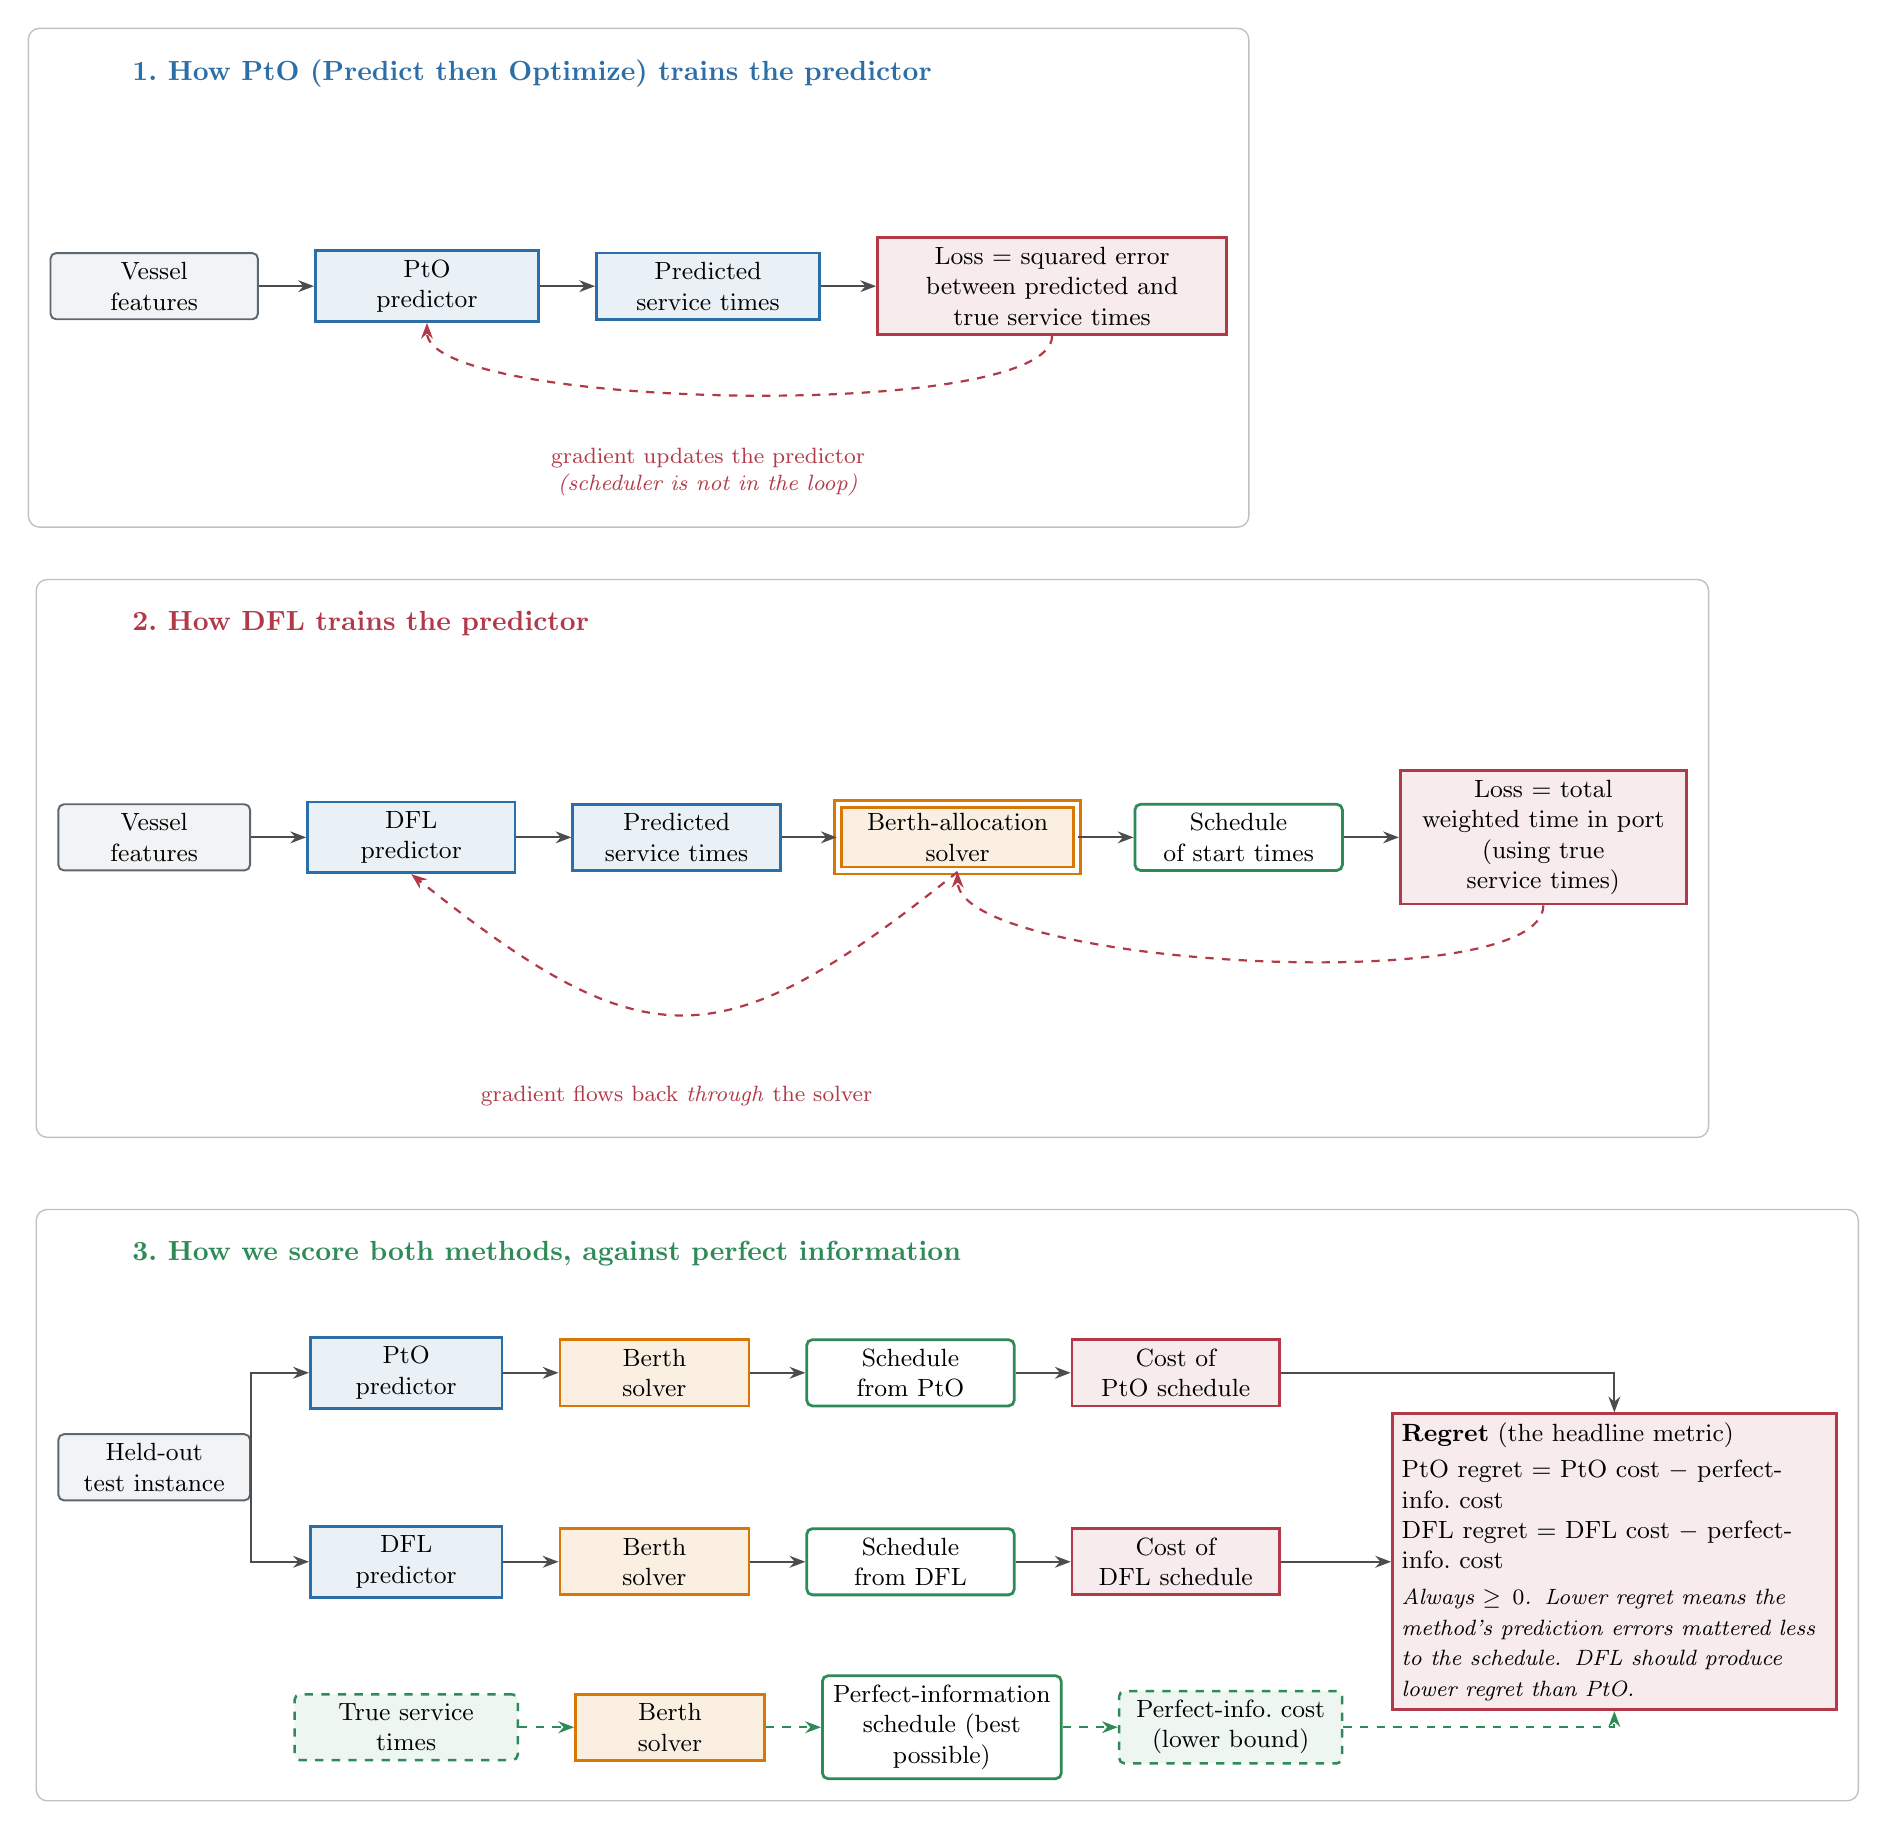
\begin{tikzpicture}[
  node distance=0.6cm and 0.7cm,
  every node/.style={font=\small}
]

% =========================================================
% BAND 1 -- PtO TRAINING
% =========================================================
\begin{scope}[local bounding box=PTOband]
  % Title and subtitle, stacked top-down with anchor=north west
  \node[font=\bfseries, predBlue, anchor=north west]
       at (-0.4, 3.0)
       {\textsc{1.\ How PtO (Predict then Optimize) trains the predictor}};

  % Node row at y=0
  \node[data, text width=2.4cm, align=center]                (xP)
       at (0, 0)
       {Vessel\\features};
  \node[pred, text width=2.6cm, align=center, right=of xP]   (fP)
       {PtO\\predictor};
  \node[pred, text width=2.6cm, align=center, right=of fP]   (yhP)
       {Predicted\\service times};
  \node[regret, text width=4.2cm, align=center, right=of yhP] (lP)
       {Loss = squared error\\between predicted and\\true service times};

  \draw[arrow] (xP)  -- (fP);
  \draw[arrow] (fP)  -- (yhP);
  \draw[arrow] (yhP) -- (lP);

  % Gradient arc below the row, label well below it
  \draw[gradArrow] (lP.south) .. controls +(0,-1.1) and +(0,-1.1) ..
                   (fP.south);
  \node[font=\footnotesize, regretRed, align=center,
        anchor=north]
       at ($(yhP.south)+(0,-1.5)$)
       {gradient updates the predictor\\
        \emph{(scheduler is not in the loop)}};
\end{scope}

\node[panel, fit=(PTOband)] (ptoBox) {};

% =========================================================
% BAND 2 -- DFL TRAINING
% =========================================================
\begin{scope}[shift={(0,-7)},
              local bounding box=DFLband]
  \node[font=\bfseries, regretRed, anchor=north west]
       at (-0.4, 3.0)
       {\textsc{2.\ How DFL trains the predictor}};

  \node[data, text width=2.2cm, align=center]                (xD)
       at (0, 0)
       {Vessel\\features};
  \node[pred, text width=2.4cm, align=center, right=of xD]   (fD)
       {DFL\\predictor};
  \node[pred, text width=2.4cm, align=center, right=of fD]   (yhD)
       {Predicted\\service times};
  \node[optbb, text width=2.8cm, align=center, right=of yhD]  (mD)
       {Berth-allocation\\solver};
  \node[decision, text width=2.4cm, align=center, right=of mD] (sD)
       {Schedule\\of start times};
  \node[regret, text width=3.4cm, align=center, right=of sD]  (lD)
       {Loss = total\\weighted time in port\\(using true\\service times)};

  \draw[arrow] (xD)  -- (fD);
  \draw[arrow] (fD)  -- (yhD);
  \draw[arrow] (yhD) -- (mD);
  \draw[arrow] (mD)  -- (sD);
  \draw[arrow] (sD)  -- (lD);

  % Two-arc gradient back through solver to predictor
  \draw[gradArrow] (lD.south) .. controls +(0,-1.2) and +(0,-1.2) ..
                   (mD.south);
  \draw[gradArrow] (mD.south) .. controls +(-3.0,-2.4) and +(3.0,-2.4) ..
                   (fD.south);
  \node[font=\footnotesize, regretRed, align=center,
        anchor=north]
       at ($(yhD.south)+(0,-2.6)$)
       {gradient flows back \emph{through} the solver};
\end{scope}

\node[panel, fit=(DFLband)] (dflBox) {};

% =========================================================
% BAND 3 -- EVALUATION
% =========================================================
\begin{scope}[shift={(0,-16)},
              local bounding box=EVALband]
  \node[font=\bfseries, truthGreen, anchor=north west]
       at (-0.4, 4.0)
       {\textsc{3.\ How we score both methods, against perfect information}};

  % xE branching point, between the PtO and DFL predictor rows
  \node[data, text width=2.2cm, align=center]   (xE) at (0, 1.0)
       {Held-out\\test instance};

  % Top row (PtO chain) at y=2.2
  \node[pred, text width=2.2cm, align=center]
       at ($(xE) + (3.2, 1.2)$)                            (fEpto)
       {PtO\\predictor};
  \node[opt, text width=2.0cm, align=center, right=of fEpto] (mEpto)
       {Berth\\solver};
  \node[decision, text width=2.4cm, align=center, right=of mEpto] (sEpto)
       {Schedule\\from PtO};
  \node[regret, text width=2.4cm, align=center, right=of sEpto] (cEpto)
       {Cost of\\PtO schedule};

  % Middle row (DFL chain) at y=0
  \node[pred, text width=2.2cm, align=center]
       at ($(xE) + (3.2, -1.2)$)                           (fEdfl)
       {DFL\\predictor};
  \node[opt, text width=2.0cm, align=center, right=of fEdfl] (mEdfl)
       {Berth\\solver};
  \node[decision, text width=2.4cm, align=center, right=of mEdfl] (sEdfl)
       {Schedule\\from DFL};
  \node[regret, text width=2.4cm, align=center, right=of sEdfl] (cEdfl)
       {Cost of\\DFL schedule};

  % Bottom row (perfect-information chain)
  \node[truth, text width=2.6cm, align=center,
        below=1.2cm of fEdfl]                              (tauE)
       {True service\\times};
  \node[opt, text width=2.0cm, align=center, right=of tauE]   (mEfi)
       {Berth\\solver};
  \node[decision, text width=2.8cm, align=center, right=of mEfi] (sEfi)
       {Perfect-information\\schedule (best possible)};
  \node[truth, text width=2.6cm, align=center, right=of sEfi] (cEfi)
       {Perfect-info.\ cost\\(lower bound)};

  % Wiring
  \draw[arrow] (xE.east) |- (fEpto.west);
  \draw[arrow] (xE.east) |- (fEdfl.west);
  \draw[arrow] (fEpto) -- (mEpto);
  \draw[arrow] (fEdfl) -- (mEdfl);
  \draw[arrow] (mEpto) -- (sEpto);
  \draw[arrow] (mEdfl) -- (sEdfl);
  \draw[arrow] (sEpto) -- (cEpto);
  \draw[arrow] (sEdfl) -- (cEdfl);

  \draw[truthArrow] (tauE) -- (mEfi);
  \draw[truthArrow] (mEfi) -- (sEfi);
  \draw[truthArrow] (sEfi) -- (cEfi);

  % Regret box on the right
  \node[regret, right=1.4cm of cEdfl, text width=5.4cm,
        minimum width=5.4cm, align=left]              (REG)
       {\textbf{Regret} (the headline metric)\\[2pt]
        PtO regret = PtO cost $-$ perfect-info.\ cost\\
        DFL regret = DFL cost $-$ perfect-info.\ cost\\[2pt]
        \footnotesize\itshape Always $\geq 0$.
        Lower regret means the method's prediction errors mattered
        less to the schedule. DFL should produce lower regret than
        PtO.};

  \draw[arrow]      (cEpto.east) -| (REG.north);
  \draw[arrow]      (cEdfl.east) -- (REG.west);
  \draw[truthArrow] (cEfi.east)  -| (REG.south);
\end{scope}

\node[panel, fit=(EVALband)] (evalBox) {};

\end{tikzpicture}%
}
\end{center}

\captionof{figure}{The whole story in one picture.  Bands 1 and 2 are
the two ways to \emph{train} the predictor.  The only difference between
them is whether the berth scheduler participates in training.  Band 3 is
how we \emph{score} both methods after training, against a
perfect-information solver that already knew the answer.  Lower regret
wins.}

\newpage

% =====================================================================
% Figure 5b -- How the test problems are built
% =====================================================================
\section*{Figure 5b.\quad How the test problems are built}

\noindent
\textbf{One test problem = one day at a small port.} Each instance is
a $\approx$ 27-hour scheduling window with 8 ships and 3 berths. The
8 ships are not all known up front --- each one has its own arrival
time within the day, and the scheduler decides which berth to send it
to and when to start serving it. The unknown the predictor learns is
each ship's \emph{service time} (how long it occupies the berth).
The numbers in the table below are the knobs of the synthetic
generator (\texttt{ports\_dfl.optim.classic\_bap.make\_classic\_problem});
the diagram below the table shows what one realized instance actually
looks like.

\vspace{0.5em}

\begin{center}
\begin{tabular}{@{}lll@{}}
\toprule
Parameter & Value & Meaning \\
\midrule
Ships per problem ($N$)        & 8                            & vessels to be scheduled in this window \\
Berths ($M$)                   & 3                            & parallel berths available \\
Scheduling window ($H$)        & $\approx 27$ h               & one day; set so total expected work $\approx$ total berth-hours \\
Contention                     & 1.0                          & expected total work / total berth capacity \\
Arrival distribution           & uniform on $[0,\,0.7H]$      & ships arrive over the first $\approx 19$ h of the window \\
Service-time distribution      & lognormal, mean $10$ h       & $\sigma$ in log-space $= 0.5$ ($\approx 50\%$ coefficient of variation) \\
Priority weights               & three classes $\{1, 2, 5\}$  & probabilities $\{60\%, 30\%, 10\%\}$; weight 5 ships count 5$\times$ in cost \\
Features per ship              & 10                           & 1 noisy estimate of $\tau$ + 1 priority weight + 8 random-noise features \\
Training problems per seed     & 80                           & used to fit the predictor \\
Test problems per seed         & 60                           & used to measure regret \\
Random seeds                   & 4 (1, 2, 3, 42)              & 240 test problems pooled across seeds \\
\bottomrule
\end{tabular}
\end{center}

\vspace{1em}

\begin{center}
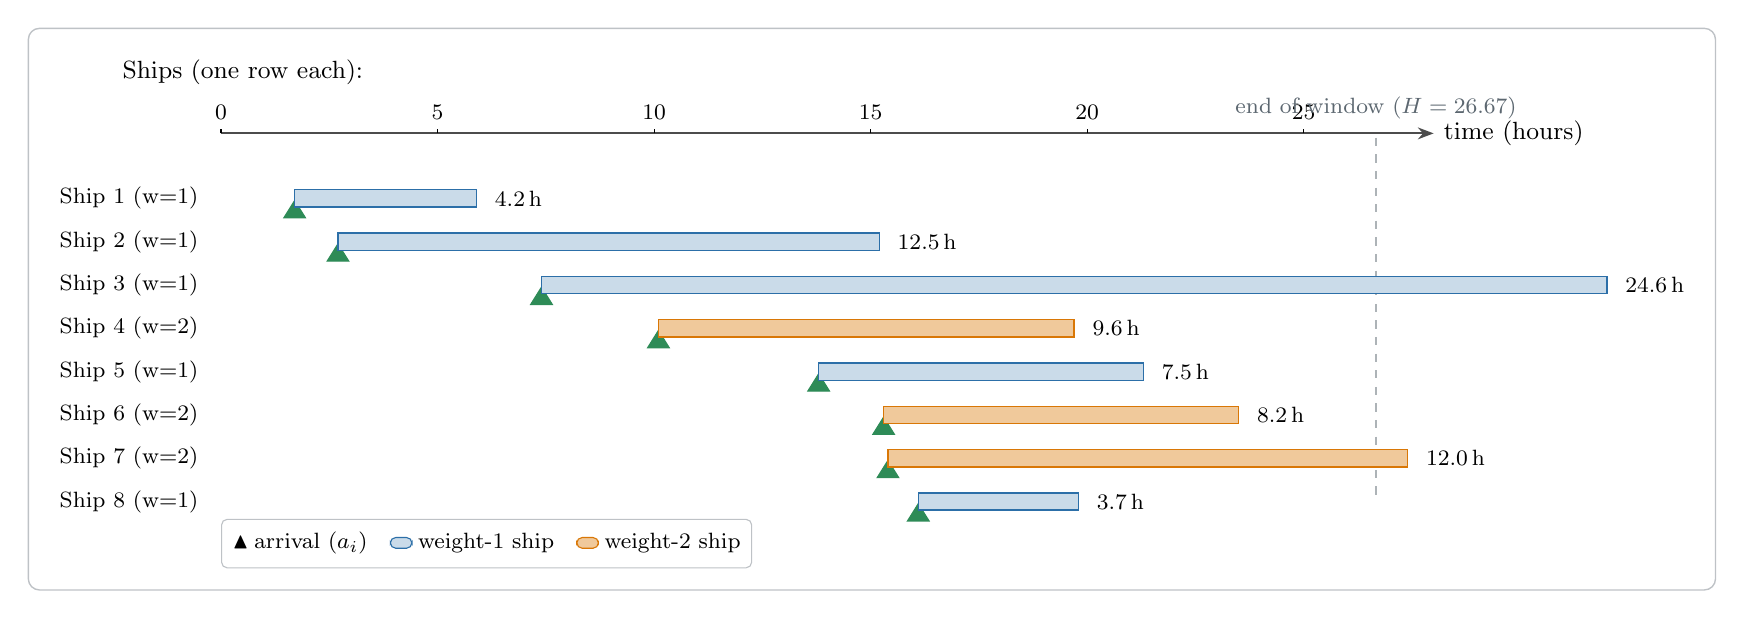
\begin{tikzpicture}[x=0.55cm, y=0.55cm]
\begin{scope}[local bounding box=fig5bcontent]
  % Time axis at the top
  \node[font=\small, anchor=south west] at (-2.5, 9.4) {Ships (one row each):};
  \draw[arrow] (0, 8.5) -- (28, 8.5) node[right, font=\small] {time (hours)};
  \foreach \t in {0, 5, 10, 15, 20, 25}{
    \draw (\t, 8.5) -- (\t, 8.6) node[above, font=\footnotesize] {\t};
  }
  % Horizon end marker
  \draw[dataGray!50, dashed] (26.67, 8.4) -- (26.67, 0);
  \node[font=\footnotesize, dataGray, anchor=south] at (26.67, 8.6)
       {end of window ($H = 26.67$)};
  % Eight ships - real data from seed=42, first test instance
  % arrivals = [1.7, 2.7, 7.4, 10.1, 13.8, 15.3, 15.4, 16.1]
  % weights  = [1,   1,   1,   2,   1,   2,   2,   1]
  % dur      = [4.18, 12.52, 24.63, 9.62, 7.46, 8.22, 12.0, 3.71]
  \foreach \i/\a/\dur/\w/\name in {
      1/1.7/4.2/1/Ship 1,
      2/2.7/12.5/1/Ship 2,
      3/7.4/24.6/1/Ship 3,
      4/10.1/9.6/2/Ship 4,
      5/13.8/7.5/1/Ship 5,
      6/15.3/8.2/2/Ship 6,
      7/15.4/12.0/2/Ship 7,
      8/16.1/3.7/1/Ship 8}{
    \pgfmathsetmacro{\y}{8 - \i}
    \node[font=\footnotesize, anchor=east] at (-0.3, \y) {\name\ (w=\w)};
    % arrival triangle
    \filldraw[truthGreen] (\a, \y-0.05) -- (\a+0.25, \y-0.45) --
                           (\a-0.25, \y-0.45) -- cycle;
    % service-time bar starting at arrival (illustration only)
    \ifnum \w=2
      \fill[optOrange!40, draw=optOrange, line width=0.5pt]
           (\a, \y-0.20) rectangle (\a+\dur, \y+0.20);
    \else
      \fill[predBlue!25, draw=predBlue, line width=0.5pt]
           (\a, \y-0.20) rectangle (\a+\dur, \y+0.20);
    \fi
    % duration value at right edge
    \node[font=\footnotesize, anchor=west]
         at (\a+\dur+0.2, \y) {\dur\,h};
  }
  % Legend
  \node[anchor=north west, draw=dataGray!40, rounded corners=2pt,
        inner sep=4pt, fill=white, font=\footnotesize]
       at (0, -0.4) {
    \begin{tabular}{@{}l@{\hspace{2pt}}l@{\hspace{8pt}}l@{\hspace{2pt}}l@{\hspace{8pt}}l@{\hspace{2pt}}l@{}}
      $\blacktriangle$ & arrival ($a_i$) &
      \tikz\fill[predBlue!25, draw=predBlue](0,0)rectangle(0.5,0.25); & weight-1 ship &
      \tikz\fill[optOrange!40, draw=optOrange](0,0)rectangle(0.5,0.25); & weight-2 ship
    \end{tabular}};
\end{scope}
\node[panel, fit=(fig5bcontent)] {};
\end{tikzpicture}
\end{center}

\captionof{figure}{One realized instance from the synthetic generator
(seed 42, first test problem). \emph{Top axis:} the 27-hour
scheduling window. \emph{Each row:} one ship. The green triangle marks
when the ship arrives at the port. The bar drawn to its right is the
ship's true service time --- the number of hours that ship will
occupy a berth once it starts being served. Bars are drawn starting
at the arrival time only to make their widths visible; the scheduler
is free to delay the start of any ship and to choose any of the three
berths. The total bar-length sums to about 82 ship-hours and the
three berths offer 80 berth-hours over the window, hence contention
$\approx 1.0$. In this particular seed there are three weight-2 ships
and five weight-1 ships; weight-5 ships have a 10\% probability so a
typical 8-ship instance has 0--1 of them.}

\newpage

% =====================================================================
% Figure 5c -- Pogancic blackbox gradient
% =====================================================================
\section*{Figure 5c.\quad The blackbox gradient (Pogan\v{c}i\'c et al., 2020)}

\noindent
\textbf{The problem.} The scheduler turns predicted service times
into a discrete schedule (which ship at which berth, in what order,
starting when). Discrete output means small changes in the input
either leave the schedule unchanged or flip it abruptly --- the
``true gradient'' of the schedule with respect to the predictions is
zero almost everywhere and undefined at the jumps. Neither helps
training a neural network.

\noindent
\textbf{The recipe.} Pogan\v{c}i\'c et al.\ get a usable gradient by
calling the scheduler \emph{twice} and taking a finite difference
between the two answers:

\begin{center}
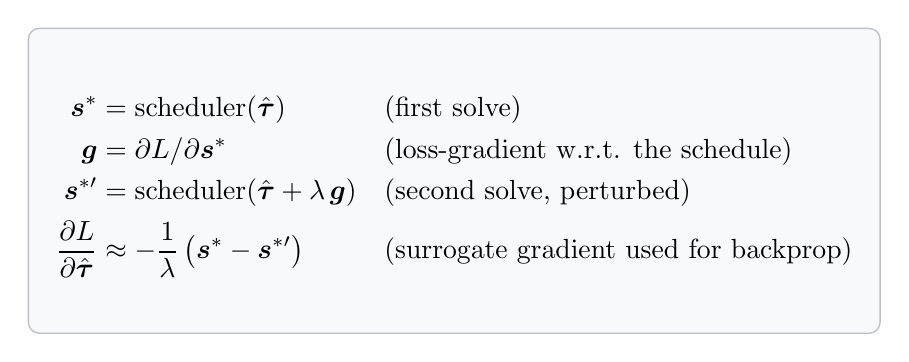
\begin{tikzpicture}
\node[panel, inner sep=10pt, fill=predBlue!4] {%
  \parbox{0.78\linewidth}{\centering
    \begin{align*}
      \boldsymbol{s}^{\ast}  &= \mathrm{scheduler}(\hat{\boldsymbol{\tau}})
            & &\text{(first solve)} \\
      \boldsymbol{g}         &= \partial L / \partial \boldsymbol{s}^{\ast}
            & &\text{(loss-gradient w.r.t. the schedule)} \\
      \boldsymbol{s}^{\ast \prime} &= \mathrm{scheduler}(\hat{\boldsymbol{\tau}} + \lambda \, \boldsymbol{g})
            & &\text{(second solve, perturbed)} \\
      \frac{\partial L}{\partial \hat{\boldsymbol{\tau}}}
          &\approx -\frac{1}{\lambda}\,\bigl(\boldsymbol{s}^{\ast} - \boldsymbol{s}^{\ast \prime}\bigr)
            & &\text{(surrogate gradient used for backprop)}
    \end{align*}}};
\end{tikzpicture}
\end{center}

\noindent
\textbf{What every symbol means.}
\begin{itemize}\setlength{\itemsep}{0pt}
  \item $\hat{\boldsymbol{\tau}}$: the model's predicted service times
        (one number per ship in the instance).
  \item $\boldsymbol{s}^{\ast}$, $\boldsymbol{s}^{\ast \prime}$: two
        schedules (vectors of start times). The first comes from the
        original predictions; the second from slightly nudged
        predictions.
  \item $\boldsymbol{g}$: how the loss would change with each ship's
        start time. Computed by standard chain rule once the loss is
        defined --- it tells us \emph{which direction} we'd like the
        schedule to move.
  \item $\lambda$: the perturbation size, a fixed positive number
        (here $\lambda = 5$). The only hyperparameter of the method.
\end{itemize}

\noindent
\textbf{Why this works (intuition).} The perturbed cost
$\hat{\boldsymbol{\tau}} + \lambda \boldsymbol{g}$ pushes the
scheduler in the direction the loss says we'd like the schedule to
move. The change in the schedule between the two solves, divided by
$\lambda$, is a finite-difference estimate of ``how the schedule
depends on $\hat{\boldsymbol{\tau}}$.'' That is the gradient we need
for backpropagation.

\noindent
\textbf{Hyperparameter trade-off.} A small $\lambda$ gives a sharper
(less biased) gradient but more variance from individual solver
corners; a large $\lambda$ is smoother but biased because it averages
over more discrete jumps. The method costs exactly \textbf{two
scheduler calls per training step}, regardless of the problem size.

\captionof{figure}{Pogan\v{c}i\'c et al.\ (2020) build a finite
difference of the scheduler's output between the original predictions
and a single targeted perturbation. The result is the gradient used
to train the predictor.}

\newpage

% =====================================================================
% Figure 5d -- Berthet Gaussian-perturbed gradient
% =====================================================================
\section*{Figure 5d.\quad The Gaussian-perturbed gradient (Berthet et al., 2020)}

\noindent
\textbf{Same problem, different fix.} Berthet et al.\ smooth the
scheduler by averaging its output over \emph{many} random
perturbations. The averaged output is a smooth function of the
predictions, with a clean gradient formula.

\noindent
\textbf{The recipe.} Choose a number of samples $K$ and a noise
magnitude $\sigma$. For each training step:

\begin{center}
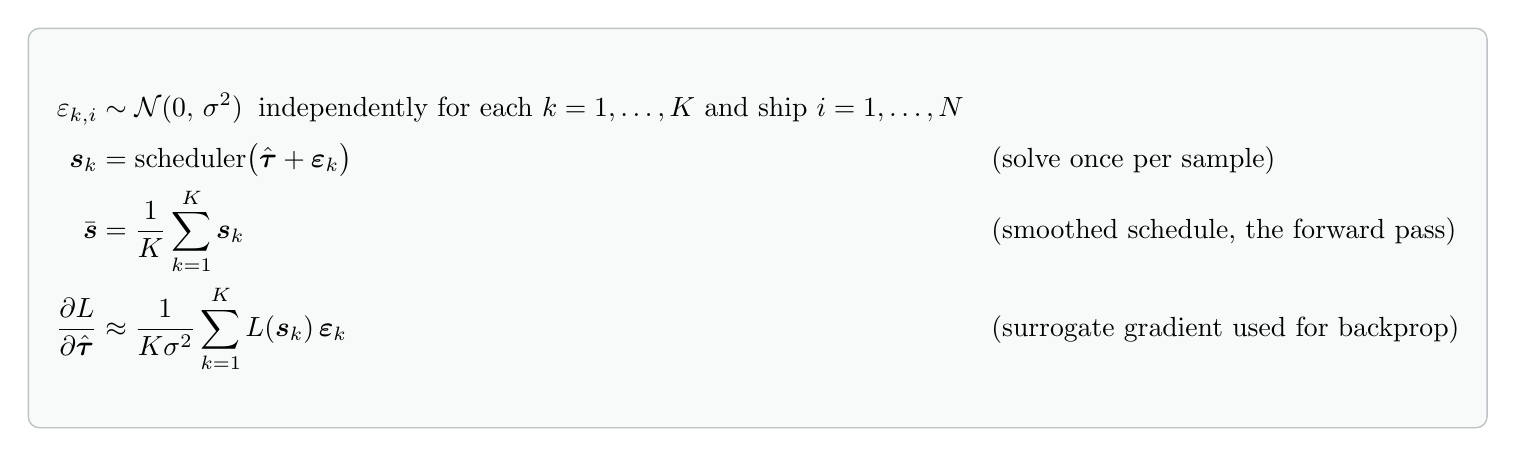
\begin{tikzpicture}
\node[panel, inner sep=10pt, fill=truthGreen!4] {%
  \parbox{0.84\linewidth}{\centering
    \begin{align*}
      \varepsilon_{k, i} &\sim \mathcal{N}(0,\,\sigma^{2})
          \;\;\text{independently for each } k = 1,\dots,K
          \text{ and ship } i = 1,\dots,N \\[2pt]
      \boldsymbol{s}_k &= \mathrm{scheduler}\bigl(\hat{\boldsymbol{\tau}} + \boldsymbol{\varepsilon}_k\bigr)
          & &\text{(solve once per sample)} \\
      \bar{\boldsymbol{s}} &= \frac{1}{K}\sum_{k=1}^{K} \boldsymbol{s}_k
          & &\text{(smoothed schedule, the forward pass)} \\
      \frac{\partial L}{\partial \hat{\boldsymbol{\tau}}}
          &\approx \frac{1}{K\sigma^{2}} \sum_{k=1}^{K} L(\boldsymbol{s}_k)\,\boldsymbol{\varepsilon}_k
          & &\text{(surrogate gradient used for backprop)}
    \end{align*}}};
\end{tikzpicture}
\end{center}

\noindent
\textbf{What every symbol means.}
\begin{itemize}\setlength{\itemsep}{0pt}
  \item $\hat{\boldsymbol{\tau}}$: predicted service times (same as
        before).
  \item $\boldsymbol{\varepsilon}_k$: a random noise vector ---
        one normal random number per ship, drawn independently with
        mean $0$ and standard deviation $\sigma$. A new vector is
        drawn for each of the $K$ samples in a step.
  \item $\sigma$: the noise magnitude (here $\sigma = 1$ h, same
        units as the predicted service times). Controls how far the
        perturbed predictions wander from the originals.
  \item $K$: the number of perturbation samples (here $K = 10$).
        Controls how noisy the gradient estimate is.
  \item $\boldsymbol{s}_k$: the schedule produced at the $k$-th
        perturbed input.
  \item $L(\boldsymbol{s}_k)$: a scalar --- the loss evaluated at
        the schedule from sample $k$.
\end{itemize}

\noindent
\textbf{Why this works (intuition).} Adding Gaussian noise smears out
the scheduler's discrete jumps: $\bar{\boldsymbol{s}}$ moves smoothly
as $\hat{\boldsymbol{\tau}}$ moves, even though each individual
$\boldsymbol{s}_k$ is discrete. The gradient formula is a
\emph{score-function} (REINFORCE-style) estimator: it weights each
noise direction by how good or bad the resulting schedule was, so on
average the predictor learns to shift $\hat{\boldsymbol{\tau}}$
toward predictions that produce low-cost schedules.

\noindent
\textbf{Hyperparameter trade-off.}
\begin{itemize}\setlength{\itemsep}{0pt}
  \item $K$: more samples $\Rightarrow$ a lower-variance gradient,
        but the training step now costs $K$ scheduler calls
        (here $\approx 10\times$ more than the blackbox method).
  \item $\sigma$: larger noise $\Rightarrow$ a smoother gradient but
        more bias (the smoothed schedule is further from the true
        argmin).
\end{itemize}

\noindent
\textbf{Compared with the blackbox method.} The blackbox method makes
\emph{one} targeted perturbation in the direction the loss says we
want the schedule to move; Berthet's method makes \emph{many random}
perturbations and lets the averaging do the smoothing. Berthet is
unbiased in the limit $K \to \infty$ (a Monte-Carlo estimate);
blackbox is a deterministic finite-difference approximation.

\captionof{figure}{Berthet et al.\ (2020) smooth the scheduler by
averaging its output over many Gaussian-perturbed inputs. The
gradient is the loss-weighted average of the noise directions ---
predictions that lead to lower-cost schedules are reinforced.}

\vspace{0.6em}

\noindent
\textbf{The two hyperparameters are $\sigma$ and $K$.}
The noise itself has no other knobs --- each ship gets an independent
draw from the same normal distribution, with no covariance between
ships. The only choices are the noise magnitude $\sigma$ and the
number of samples $K$.

\vspace{0.4em}

\noindent
\textbf{How $\sigma$ and $K$ are tuned in practice.}
\begin{itemize}\setlength{\itemsep}{0pt}
  \item \textbf{Default values.} The PyEPO library (the de-facto
        standard implementation) ships with $\sigma{=}1$ and $K{=}10$.
        Used as-is in many DFL papers and in this project.
  \item \textbf{Scale $\sigma$ to the cost vector.} $\sigma$ is added
        to $\hat{\boldsymbol{\tau}}$ \emph{in the same units as
        $\hat{\boldsymbol{\tau}}$}. Practitioners either (i)
        standardize the cost so $\sigma{=}1$ is meaningful or (ii)
        sweep $\sigma \in \{0.1,\,0.5,\,1,\,2\}$. Too small a $\sigma$
        leaves the gradient zero (no perturbed sample crosses a
        scheduler decision boundary); too large washes out the signal.
  \item \textbf{Pick $\sigma$ by grid search on validation regret.}
        Mandi et al.'s JAIR 2024 DFL survey reports this as the most
        common protocol. Bayesian tuning is rare.
  \item \textbf{$K$ trades variance for solver calls.} Variance of the
        gradient $\propto 1/K$. The training step costs $K$ scheduler
        calls. Common values are $K \in \{1,3,10\}$; expensive solvers
        favour small $K$, cheap solvers favour large $K$.
  \item \textbf{Recipe.} Pick the smallest $\sigma$ that gives a
        non-zero gradient on most samples, then raise $K$ only until
        the validation regret stops improving.
\end{itemize}

\vspace{0.4em}

\noindent
\textbf{Picking $\sigma$ from the BAP structure.}
The rules above are problem-agnostic --- they tune $\sigma$ against
training stability, not against the BAP's own decision granularity.
When the BAP carries time windows, the perturbation has a natural
operational scale: the \emph{slack} between a vessel's predicted
completion and its deadline. Perturbations smaller than the slack
rarely flip a decision; perturbations larger than the slack reliably
do. Three rules tie $\sigma$ to that structure:

\begin{itemize}\setlength{\itemsep}{0pt}
  \item \textbf{Median window width.} $\sigma = \mathrm{median}_i\,
        (b_i - a_i)$ across the training instances. One scalar, fixed
        across training; reads as ``size the perturbation to the
        typical scheduling window.'' Cleanest option for a paper
        headline.
  \item \textbf{Median slack.} $\sigma = \mathrm{median}_i\,
        (b_i - a_i - \hat{\tau}_i)$, recomputed per instance. Adapts
        to the tightness of the current problem --- $\sigma$ shrinks
        when windows are crowded, grows when they are loose.
  \item \textbf{Per-vessel slack (anisotropic).} $\sigma_i = \alpha
        \cdot \mathrm{slack}_i$ with $\alpha \in [0.5,\,1]$. Each ship
        gets noise proportional to its own room before the deadline:
        ships near their cliffs get small, targeted perturbations;
        ships with room to spare get broad ones. Floor $\sigma_i$ at a
        small positive value when $\mathrm{slack}_i \leq 0$ so the
        vessels DFL most needs to learn from are not skipped. Loses
        Berthet's clean isotropic theory but matches the BAP's
        per-vessel heterogeneity.
\end{itemize}

\noindent
\emph{Justification.} Berthet's $\sigma$ is correct when it matches
the scale of the LP's piecewise-linearity. In BAP with time windows
that scale is set by the deadline slack: cost cliffs sit exactly at
$s_i + \tau_i = b_i$, so the right smoothing radius is the typical
distance to that boundary.

\vspace{0.4em}

\noindent
\textit{Sources.} Berthet et al., NeurIPS 2020 (arXiv:2002.08676);
PyEPO source \texttt{pkg/pyepo/func/perturbed.py}; Tang \& Khalil,
\emph{PyEPO} (MPC 2024, arXiv:2206.14234); Mandi et al., JAIR 2024
DFL survey (arXiv:2307.13565).

\newpage

% =====================================================================
% Figure 6 -- Sample results
% =====================================================================
\section*{Figure 6.\quad Where DFL pays off
\;\textnormal{\normalsize(linear regression predictor trained with schedule-cost gradients)}}

\noindent
\textbf{What we plot.} For each test instance (8 ships to schedule on
3 berths) we compare two costs: the cost of the schedule the method's
predictions produce, and the cost a perfect-information scheduler
(one that already knew the true service times) would have produced.
The gap between the two is the \emph{regret}. Low regret means the
method's prediction errors did not really hurt the schedule. Regret
is measured in weighted ship-hours, the same units as the scheduler's
objective: each ship's completion time multiplied by its priority
weight.

\textbf{Setup.} 8 ships per instance, 3 berths, three-class priority
weights \{1, 2, 5\} (about 10\% of ships are 5$\times$ as important
as the rest). Three methods, all using the same linear predictor and
the same training data:
\begin{itemize}\setlength{\itemsep}{0pt}
  \item \textbf{PtO} -- predictor trained on prediction error (the
        standard recipe).
  \item \textbf{DFL Blackbox} -- predictor trained on schedule cost,
        gradient via Pogan\v{c}i\'c et al.\ (2020).
  \item \textbf{DFL Perturbed} -- predictor trained on schedule cost,
        gradient via Berthet et al.\ (2020).
\end{itemize}

\vspace{0.5em}

\begin{center}
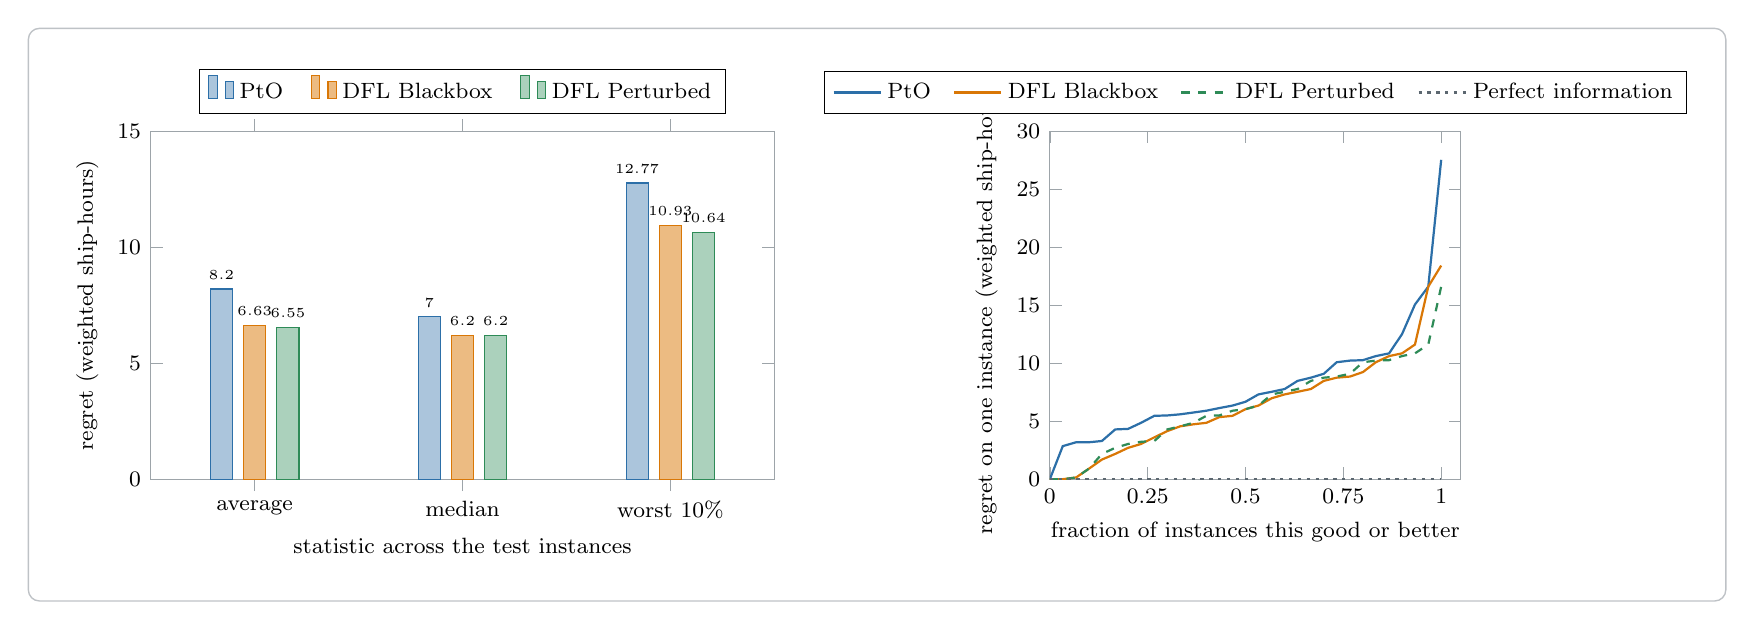
\begin{tikzpicture}
\begin{scope}[local bounding box=fig6content]
  \begin{axis}[
    name=bars,
    width=9.5cm, height=6.0cm,
    ybar=4pt, bar width=8pt,
    ymin=0, ymax=15,
    ylabel={regret (weighted ship-hours)},
    xlabel={statistic across the test instances},
    symbolic x coords={mean,median,p90},
    xtick=data,
    xticklabels={average,median,worst 10\%},
    enlarge x limits=0.25,
    legend style={at={(0.5,1.05)}, anchor=south,
                  font=\footnotesize,
                  /tikz/every even column/.append style={column sep=8pt}},
    legend columns=3,
    nodes near coords, nodes near coords style={font=\tiny},
    tick label style={font=\footnotesize},
    label style={font=\footnotesize},
    axis line style={draw=dataGray!60},
    tick style={draw=dataGray!60},
  ]
    \addplot[fill=predBlue!40, draw=predBlue]
            coordinates {(mean,8.20) (median,7.00) (p90,12.77)};
    \addplot[fill=optOrange!50, draw=optOrange]
            coordinates {(mean,6.63) (median,6.20) (p90,10.93)};
    \addplot[fill=truthGreen!40, draw=truthGreen]
            coordinates {(mean,6.55) (median,6.20) (p90,10.64)};
    \legend{PtO, DFL Blackbox, DFL Perturbed}
  \end{axis}

  \begin{axis}[
    at={(bars.east)}, anchor=west, xshift=3.5cm,
    width=6.8cm, height=6.0cm,
    xmin=0, xmax=1.05, ymin=0, ymax=30,
    xtick={0,0.25,0.5,0.75,1},
    xticklabel style={/pgf/number format/.cd, fixed, precision=2},
    ytick={0,5,10,15,20,25,30},
    xlabel={fraction of instances this good or better},
    ylabel={regret on one instance (weighted ship-hours)},
    legend style={at={(0.5,1.05)}, anchor=south, font=\footnotesize,
                  /tikz/every even column/.append style={column sep=6pt}},
    legend columns=4,
    tick label style={font=\footnotesize},
    label style={font=\footnotesize},
    axis line style={draw=dataGray!60},
    tick style={draw=dataGray!60},
  ]
    \addplot[predBlue, thick] coordinates {
      (0,0) (0.033,2.852) (0.067,3.186) (0.1,3.186) (0.133,3.295)
      (0.167,4.292) (0.2,4.34) (0.233,4.863) (0.267,5.467)
      (0.3,5.498) (0.333,5.595) (0.367,5.752) (0.4,5.907)
      (0.433,6.135) (0.467,6.351) (0.5,6.679) (0.533,7.313)
      (0.567,7.538) (0.6,7.776) (0.633,8.479) (0.667,8.755)
      (0.7,9.091) (0.733,10.087) (0.767,10.227) (0.8,10.265)
      (0.833,10.617) (0.867,10.853) (0.9,12.514) (0.933,15.064)
      (0.967,16.606) (1,27.54)
    };
    \addplot[optOrange, thick] coordinates {
      (0,0) (0.033,0) (0.067,0.147) (0.1,0.911) (0.133,1.693)
      (0.167,2.181) (0.2,2.705) (0.233,3.039) (0.267,3.61)
      (0.3,4.148) (0.333,4.56) (0.367,4.735) (0.4,4.863)
      (0.433,5.352) (0.467,5.467) (0.5,6.039) (0.533,6.351)
      (0.567,6.982) (0.6,7.313) (0.633,7.538) (0.667,7.776)
      (0.7,8.479) (0.733,8.755) (0.767,8.852) (0.8,9.237)
      (0.833,10.087) (0.867,10.617) (0.9,10.853) (0.933,11.611)
      (0.967,16.606) (1,18.421)
    };
    \addplot[truthGreen, thick, dashed] coordinates {
      (0,0) (0.033,0) (0.067,0.147) (0.1,0.911) (0.133,2.181)
      (0.167,2.705) (0.2,3.039) (0.233,3.227) (0.267,3.295)
      (0.3,4.292) (0.333,4.56) (0.367,4.863) (0.4,5.467)
      (0.433,5.498) (0.467,5.907) (0.5,6.039) (0.533,6.351)
      (0.567,7.313) (0.6,7.538) (0.633,7.776) (0.667,8.479)
      (0.7,8.755) (0.733,8.852) (0.767,9.091) (0.8,10.087)
      (0.833,10.227) (0.867,10.265) (0.9,10.617) (0.933,10.853)
      (0.967,11.611) (1,16.606)
    };
    % Perfect-information: regret = 0 at every quantile (horizontal at y=0)
    \addplot[dataGray, very thick, dotted] coordinates {
      (0, 0) (1, 0)
    };
    \legend{PtO, DFL Blackbox, DFL Perturbed, Perfect information}
  \end{axis}
\end{scope}
\node[panel, fit=(fig6content), inner sep=14pt] {};
\end{tikzpicture}
\end{center}


\newpage

% =====================================================================
% Notation
% =====================================================================
\section*{Notation cheat-sheet}

\begin{center}
\begin{tabular}{@{}ll@{}}
\toprule
Symbol & Meaning \\
\midrule
$\tau_i$            & true service time for vessel $i$ (target, unknown ex ante). \\
$\hat{\tau}_i$      & predicted service time from $f_\theta$. \\
$x_{ib}$            & binary, $1$ if vessel $i$ is assigned to berth $b$. \\
$s_i$               & start time of vessel $i$ at its berth ($s_i \geq a_i$). \\
$z_{ijb}$           & binary precedence: $1$ if $i$ precedes $j$ at berth $b$. \\
$a_i$               & arrival time of vessel $i$. \\
$w_i$               & priority weight of vessel $i$. \\
$\lambda$           & blackbox interpolation strength; $\lambda{=}5$ here. \\
FI                  & full-information schedule: MILP on the true $\tau$. \\
$s^\ast$            & start times from the MILP at $\hat{\tau}$ (training time). \\
$f_\theta$          & predictor; here \texttt{nn.Linear($d,1$)} (same architecture in both). \\
$L_{\mathrm{PtO}}$  & $\lVert\hat{\tau}-\tau\rVert_2^2$. \\
$L_{\mathrm{DFL}}$  & $\sum_i w_i(s^\ast_i + \tau_i)$. \\
$C_{\mathrm{PtO}},\,C_{\mathrm{DFL}},\,C_{\mathrm{FI}}$
                    & evaluation-time schedule costs (always on true $\tau$). \\
Regret              & $C_{\mathrm{method}} - C_{\mathrm{FI}} \geq 0$.\;\; Lower is better. \\
\bottomrule
\end{tabular}
\end{center}

\vspace{1em}

\noindent\textit{Source code, all under \texttt{prediction\_models/}:}

\begin{itemize}\setlength{\itemsep}{0pt}\small
  \item \texttt{src/ports\_dfl/optim/discrete\_bap.py} \;(MILP, objective, big-M, mutable $\tau$).
  \item \texttt{src/ports\_dfl/optim/classic\_bap.py} \;(synthetic instance generator used in Figure 5b).
  \item \texttt{src/ports\_dfl/train/pto.py} \;($L_{\mathrm{PtO}}$, AdamW + Cosine).
  \item \texttt{src/ports\_dfl/train/dfl\_blackbox.py} \;(Pogan\v{c}i\'c blackbox gradient, $\lambda$).
  \item \texttt{src/ports\_dfl/train/dfl\_perturbed.py} \;(Berthet Gaussian-perturbed gradient, $\sigma$, $K$).
\end{itemize}

\end{document}
